В секции представлены разработанные игры, использующие современные нейросетевые технологии для 
персонального обучения. Выбор направления был выполнен с учетом растущих возможностей больших языковых моделей. 
В качестве предмета обучения были выбраны стратегические игры, развивающие навыки долгосрочного планирования и критического мышления. 
Также  было исследовано применение диффузионных моделей для растрового рисования, позволяющее отработать навыки передачи
структуры и природы объектов.

Современные большие языковые модели пока не способны к полноценному ведению игры. В работе \cite{Adam2024} проведен анализ силы игры ассистента ChatGPT 
путем сравнения с шахматной программой Stockfish. Статистические исследования показывают, что текущий уровень игры модели соответствует рейтингу Эло 1600
\cite{elo1967proposed}. Это начальный уровень игрока в шахматы. Исследователи также отмечают неспособность ассистента к строгому исполнению правил игры
и наблюдают противоречия в стратегии даже в коротком отрезке партии.

Исходя из текущих возможностей был предложен гибридный подход, заключающийся в совмещение языковой модели с 
открытой шахматной программой StockFish \cite{acher2016large}. В такой постановке интеллектуальный ассистент отвечает на вопросы 
пользователя по ходу игры и рассказывает о возможных стратегических решениях, исходя из ситуации на доске. 
Шахматная программа задает уровень оппонента и выдает информацию для обновления рейтинга. Обновление выполняется в соответствии с моделью Эло, 
в зависимости от уровня игры оппонента по правилу:
\begin{equation}
    x_{i+1}=x_i + K(\beta) \left[X_i-P(X_i=1)\right],
\end{equation}
где $P(X_i=1)$ задает вероятность победы в игре.

Алгоритм базовой игры может быть описан как последовательность шагов:
\begin{enumerate}
    \item пользователь начинает игру;
    \item пользователь по ходу игры консультируется с ассистентом, и при необходимости изменяет сложность;
    \item ассистент отслеживает результаты игры и обновляет рейтинг. Пользователь может запрашивать советы.
\end{enumerate}

Для поощрения настойчивости и развития интереса к игре была разработана система достижений, включающая как количественную оценку прогресса, 
так и выполнение нестандартных задач. Правила получения награды определяются порогом отсечки с помощью алгоритма, описанного в \ref{badge}.
Такая система поощряет соревновательный дух.

\begin{figure}[h]
    \centering
    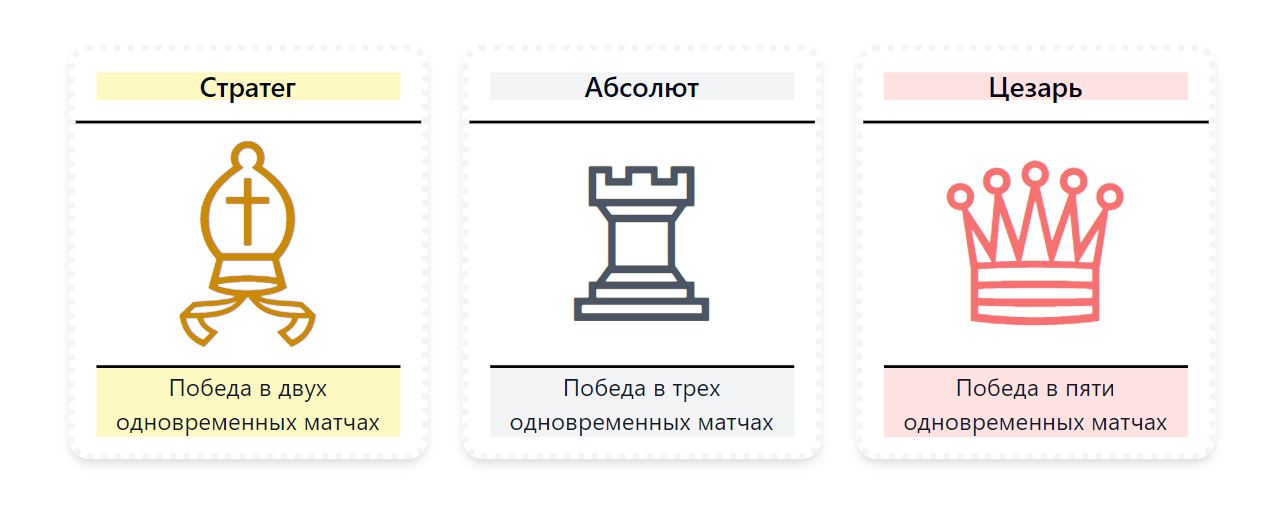
\includegraphics[width=0.7\textwidth]{assets/work/games/achieve.png}
    \caption{Достижение на примере награды за победу в сеансе одновременной игры}
    \label{achievement}
\end{figure}

Разработка игры по рисованию была выполнена с использованием открытой диффузионной модели \ref{diffusion},
составляющей рисунок по текстовому запросу. Для простоты выполнения рисунка предложено выполнение мозаики из
пикселей, представляющих базовый элемент растровой сетки изображения. Адаптация базовой модели для стилизации
рисунка выполняется с помощью открытого низкорангового адаптера. Исходный запрос для модели должен быть 
сформулирован на английском языке, лаконично описывать объекты на изображении и обстановку. 
В силу случайности генерации пользователь может подобрать для себя наиболее интересный вариант изображения.
Сложность рисунка определяется наличием фона, декораций и сложностью композиции. 

Алгоритм выполнения рисунка состоит из трех последовательных этапов:
\begin{enumerate}
    \item пользователь вводит описание желаемого предмета на русском языке;
    \item ассистент переводит запрос на английский язык с учетом его рейтинга и предоставляет пользователю выбор из заданных рисунков;
    \item кодировщик сранивает рисунок с исходным изображением и определяет балл для обновления рейтинга.
\end{enumerate}

Модель дополнительно снабжена фильтром цензуры, позволяющем исключать изображения не соответствующие этике \cite{radford2021learning}.
Уровень сложности регулируется путем изменения композиции и наличия фона.
\begin{figure}[h]
    \centering
    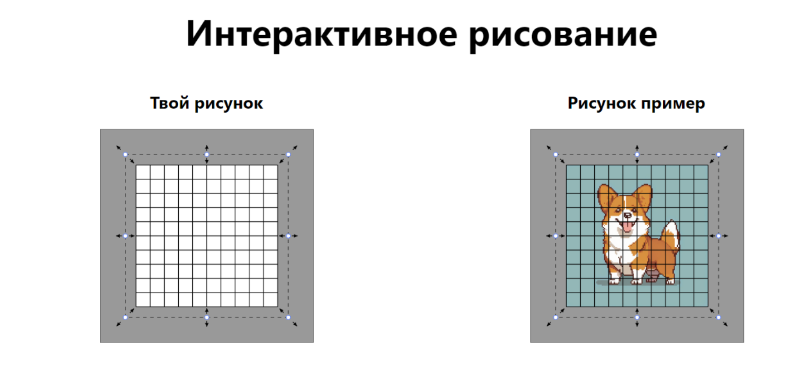
\includegraphics[width=0.7\textwidth]{assets/work/games/draw.excalidraw.png}
    \caption{Рисунок выполняется путем сопоставления результата с опорным изображением.}
    \label{draw}
\end{figure}
